% Teilaufgabe 11
\newpage
\section{Möglichkeiten der Signal-Rausch Verbesserung}
\label{sec:verbesserung}
\subsection{Filter}
\label{sub:filter}
\subsection{Mittelung}
\label{sub:mittelung}
\newpage
\subsection{Lock-In Verstärker}
\label{sub:lockin}
Ein Lock-In Verstärker ist ein Detektor zum Auflösen von kleinen Wechselspannungssignalen bis zu ein paar nV. Dabei ist eine akkurate Messung des Signals, welches 1000fach stärkeres Rauschen besitzt, möglich. Es kommt dafür einen sogenannte phasensensitive Detektion zum Einsatz, um eine bestimmte Komponente des Signals bei einer bestimmten Referenzfrequenz $f_{r}$ und Phase $\Theta_{r}$ zu bestimmen. Dabei wird Rauschen, welches nicht auf der Referenzfrequenz liegt, herausgefiltert und trägt nicht mehr zum Signal bei.
\subsection*{Phasensensitive Detektion}
Beim Lock-In wird wie oben erwähnt eine Referenzfrequenz benötigt. Diese Frequenz wird meistens durch das Experiment vorgegeben (z.B. Funktionsgenerator) und der Lock-In detektiert die Antwort des Experiments bei dieser Referenzfrequenz. In Abbildung \ref{image:signalRef} sind schematisch die jeweiligen Signale gezeigt. Als Referenzsignal wird eine Rechteckschwingung mit $f_{r}$ verwendet und das Experiment selbst wird von einer Sinusschwingung (Input-Signal) mit Funktion $s(t)=U_{s}\sin(\omega_{r}t + \Theta_{s})$ mit $\omega_{r}=2\pi f_{r}$, Amplitude $U_s$ und Phasenverschiebung $\Theta_{s}$ angeregt. Der Lock-In Verstärker erzeugt dann selbst eine Sinusschwingung mit Frequenz $f_l$ und der Funktion $l(t) = \sin(\omega_{l}t + \Theta_{r})$ mit $\omega_{l}=2\pi f_{l}$ als Signal, das Lock-In-Signal.
\begin{center}
    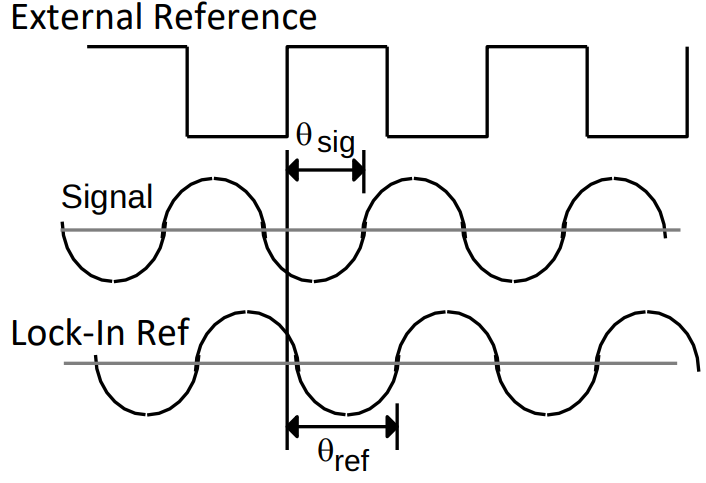
\includegraphics[scale = 0.3]{SignalLockIn.png}
    \captionof{figure}{Signale bei einem Lock-In Verstärker \citep{lockin}}
    \label{image:signalRef}
\end{center}
Nun multipliziert der Lock-In Verstärker das Input-Signal und das Lock-In-Signal mit einem phasensensitiven Detektor (PSD) oder einem Multiplikator. Daraus folgt mit Anwendung des Additionstheorems des Sinus:
\begin{gather}
    \begin{aligned}
        s_{x} &= s(t)\cdot l(t) = U_{s}\sin(\omega_{r}t + \Theta_{s}) \cdot \sin(\omega_{l}t + \Theta_{r})\\
                &= \frac{U_{s}}{2}\left[\cos((\omega_{r}-\omega_{l}) + (\Theta_s - \Theta_r)) + \cos((\omega_{r}+\omega_{l}) + (\Theta_s + \Theta_r))\right]
    \end{aligned}
\end{gather}
Damit ist das Output-Signal $s_x$ zwei Wechselspannungssignale mit unterschiedlichen Frequenzen. Dieses Signal wird durch einen Tiefpassfilter geschickt, welcher alle Wechselspannungssignale eliminiert.\\ Wenn $\omega_r = \omega_l$ ist, ist das Signal mit der Differenz der Frequenz ein Gleichspannungssignal und wird somit nicht gefiltert. Der neue PSD Output ist dann:
\begin{gather}
    s_{x} = \frac{U_s}{2} \cos(\Theta_s-\Theta_r) = \frac{U_s}{2} \cos(\Delta\Theta)  
\end{gather}
Bei einem Phasenunterschied von $\Delta\Theta = 0$ lässt sich hierbei das Maximum der Amplitude messen ($\frac{U_s}{2}$) und bei $\Delta\Theta = \frac{\pi}{2}$ misst man überhaupt kein Output-Signal mehr. Solche Lock-In Verstärker mit nur einem PSD werden auch Einphasen-Lock-In genannt. Man kann aber auch ein zweites Lock-In-Signal mit Cosinusschwinung verwenden und dieses mit einem zweiten PSD mit dem Input-Signal multiplizieren. Mit dem selben Prozess wie zuvor erhält man die Beziehung:
\begin{gather}
    s_{y} = \frac{U_s}{2} \sin(\Delta\Theta) 
\end{gather} 
Das Output $s_x$ heißt \enquote{in Phase}-Komponente und $s_y$ die \enquote{Quadratur}-Komponente, weil bei $\Delta\Theta = 0$ ist $s_y = 0$ und $s_x$ misst das Input-Signal.\\

Weiterhin kann man mit $s_x$ und $s_y$ wie folgt die Amplitude des Output-Signals bestimmen:
\begin{gather}
    A = (s_x^2 + s_y^2)^{\frac{1}{2}} = \frac{U_s}{2}
\end{gather}
\subsection*{Was wird mit einem Lock-In gemessen?}
Ein Lock-In Verstärker misst aufgrund der Multiplikation mit einer Sinusschwingung (Cosinusschwinung) den ersten Term der Fourier-Reihe des Input-Signals bei der Referenzfrequenz $f_r$. Dabei ist aber zu beachten, dass auch Rauschen, welches bei der Referenzfrequenz auftritt, mit gemessen wird und gegebenenfalls abgezogen werden muss. In Abbildung \ref{image:Block} ist zusätzlich der Aufbau des Lock-In Verstärkers dargestellt \citep{lockin}.
\newpage
\begin{center}
    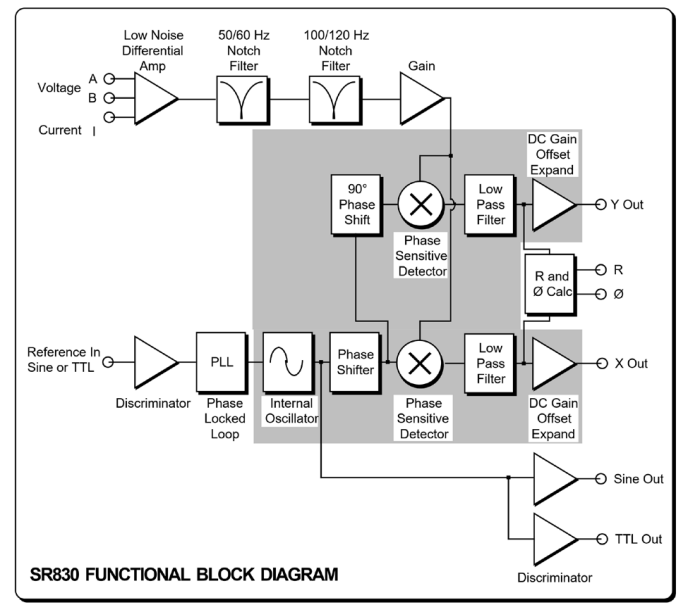
\includegraphics[scale = 0.6]{BLockdiagrammLockIn.png}
    \captionof{figure}{Blockdiagramm Lock-In Verstärker \citep{lockin}}
    \label{image:Block}
\end{center}

\newpage
\section{Leistungspegel}
Der Leistungspegel $L_p$ gibt das 10fache logarithmische Verhältnis zwischen Nutzleistung $P$ und Bezugsleistung $P_0$ in \si{\deci\bel} an und ist definiert als:
\begin{gather}
    L_P = 10 \log_{10}\left(\frac{P}{P_0}\right)
    \label{eq:pegel}
\end{gather}
In diesem Versuch ist vom Interesse den Leistungspegel der Spannungen $L_U$ anzugeben. Dafür wird die Formel $P = U \cdot I$ mit dem ohmischen Gesetz $R = \frac{U}{I}$ umgestellt zu $P = \frac{U^2}{R}$ und in Gleichung (\ref{eq:pegel}) eingesetzt. Somit erhält man:
\begin{gather}
    L_U = 10 \log_{10}\left(\frac{U^2}{U_0^2}\right) = 20 \log_{10}\left(\frac{U}{U_0}\right)
\end{gather}
Damit entspricht der Leistungspegel der Spannungen das doppelte des herkömmlich definierten Leistungspegel \citep{electronik}.\\
Um das Verständnis zu vertiefen werden noch einige bestimmte Verhältnisse zu charakteristischen \si{\deci\bel} angegeben:
\begin{center}
    \begin{tabular}{c | c c}
        $L$/dB & $\frac{P}{P_0}$ & $\frac{U}{U_0}$\\
        \hline
        $-n\cdot10$ & $1\cdot10^{-n}$ &  $1\cdot10^{-n/2}$ \\
        -20 & 1/100 & 1/10 \\
        -10 & 1/10 & 1/$\sqrt{10}$ \\
        -6 & 1/4 & 1/2\\
        -3 & 1/2 & 1/$\sqrt{2}$\\
        0 & 1 & 1\\
        3 & 2 & $\sqrt{2}$\\
        6 & 4 & 2\\
        10 & 10 & $\sqrt{10}$ \\
        20 & 100 & 10 \\
        $n\cdot10$ & $1\cdot10^{n}$ &  $1\cdot10^{n/2}$ \\
    \end{tabular}
    \captionof{table}{Leistungspegel und zugehörige Verhältnisse}
    \label{tab:pegel}
\end{center}
In Tabelle \ref{tab:pegel} lässt sich sehr gut die Verdopplungsregel des Leistungspegel erkennen. Dabei steigt der Pegel um 3dB an (bei $L_U$ um 6dB), wenn man das Verhältnis verdoppelt. Dies hat damit zu tun, dass der 10er-Logarithmus von 2 ungefähr 0.3 ist und dieser mit der Multiplikation von 10 nach der Gleichung (\ref{eq:pegel}) dann 3dB ergibt.
\newpage
\section{Abtasttheorem}
Das Abtasttheorem besagt, dass aus den Abtastwerten das ursprüngliche Signal (kontinuierlich) fehlerfrei rekonstruiert werden kann, wenn die Abtastfrequenz mindestens doppelt so groß ist wie die höchste Signalfrequenz $f_{max}$. 
\begin{gather}
    f \geq 2\cdot f_{max}
\end{gather} 
Die Frequenz $2f_{max}$ wird als \textit{Nyquist-Frequenz} bezeichnet. Aus dem Abtasttheorem folgt auch, dass das Spektrum des Signals \textit{bandbegrenzt} ist \citep{praktikum}.
\section{Fouriertransformation und Schnelle Fouriertransformation}
Bei einer Fouriertransformation wird ein gegebenes Signal (ggf. eine Funktion) komplett in den Frequenzraum transformiert, dabei wird ein Integral von $-\infty$ bis $\infty$ ausgewertet. Der Rechenaufwand einer Fouriertransformation ist in der Regel in der Praxis sehr hoch, weswegen meist eine Schnelle Fouriertransformation (engl. Fast Fourier Transformation (FFT)) durchgeführt wird. Unter einer FFT versteht man eine effiziente Realisierung der Diskrete Fouriertransformation (DFT), mit der redundante Rechenschritte vermieden werden. Bei einer DFT wird nur ein abgetastetes Signal in den Frequenzraum überführt.Der Rechenaufwand von $N^2$ bei einer DFT verringert sich dann  bei einer FFT zu $\approx N\log_2\left(N\right)$ \citep{praktikum}.
\section{Fourier-Reihe und Effektivspannung}
\label{sec:fourierseries}
\subsection*{Allgemeines zur Fourier-Reihe und Effektivspannungen}
\label{sub:fourierseriesAllgemein}
Eine Fourier-Reihe zerlegt eine gegeben periodische Funktion in ihre jeweiligen Sinus und Cosinusanteile. Die reelle Fourier-Reihe einer bestimmten $T$-periodischen Funktion lässt sich mit den folgenden Formeln berechnen:
\begin{gather}
    f(t) = \frac{a_0}{2} + \sum^{\infty}_{k=1} \left[a_k \sin(k\frac{2\pi}{T} t) +b_k \cos(k\frac{2\pi}{T} t)\right]\\
    a_k = \frac{2}{T} \int^{\frac{T}{2}}_{-\frac{T}{2}} f(t)\cos(k \frac{2\pi}{T} t)dt\\
    b_k = \frac{2}{T} \int^{\frac{T}{2}}_{-\frac{T}{2}} f(t)\sin(k \frac{2\pi}{T} t)dt
\end{gather}
Dabei sind die Grenzen der Integrale von $-\frac{T}{2}$ bis $\frac{T}{2}$ nicht fest, sie können verschoben werden. Es ist aber wichtig, dass über eine Periode integriert wird in diesem Fall über eine komplette Periodendauer $T$ \citep{praktikum}.\\

Um die effektiven Spannungswerte der jeweiligen Schwingungsform zu bestimmen, bildet man das sogenannte \enquote{Quadratische Mittel}. Dieses ist wie folgt definiert:
\begin{gather}
    U_{eff} = \sqrt{\frac{1}{T}\int^T_0 f(t)^2 dt}
\end{gather}
Hierbei ist es wieder zu erwähnen, dass die Grenzen der Integration nicht fest sind, aber die Integration über eine Periodenlänge erfolgen muss \citep{messtechnik}.\\

Die detaillierteren Berechnungen zu jeder Schwingungsform lassen sich in Anhang \ref{app:Berechnung} nachlesen.

\subsection*{Sinusschwingung}
\label{sub:sinus}
Der Fall der Sinusschwingung ist besonders einfach, da wie vorangegangen erwähnt, die Fourier-Reihe eine periodische Funktion in ihre Sinus und Cosinusanteile zerlegt. Daraus folgt die Fourier-Reihe der Sinusschwingung ist die Sinusschwingung selbst und kann somit trivial angegeben werden als:
\begin{gather}
    \boxed{f(t) = U_0\sin(\frac{2\pi}{T} t)}
\end{gather}
Die Effektivspannungen der Sinusschwingung:
\begin{gather}
    \boxed{U_{eff}=\frac{U_0}{\sqrt{2}}}
\end{gather}

\subsection*{Rechteckschwingung}
\label{sub:square}
Als nächstes wird die Fourier-Reihe der Rechteckschwingung bestimmt. Diese hat die Form:
\begin{gather}
    f(t) = 
    \begin{cases}
        +U_0, & 0 \leq t \leq \frac{T}{2} \\
        -U_0, & \frac{T}{2} \leq t \leq T \\
    \end{cases}
\end{gather}
Da die Funktion der Rechteckschwingung punktsymmetrisch zum Ursprung ist, fallen alle Cosinusanteile weg, da $a_k = 0$. Somit muss nur $b_k$ wie folgt berechnet werden:
\begin{gather}
    b_k =
    \begin{cases}
        0, & k~\text{gerade}\\
        \frac{4U_0}{\pi}\frac{1}{2k-1}, & k~\text{ungerade}\\
    \end{cases}
\end{gather} 
Es werden nur noch Terme mit ungeraden $k$ betrachtet und man erhält:
\begin{gather}
    \boxed{f(t) = \frac{4U_0}{\pi} \sum^{\infty}_{k=1} \frac{1}{2k-1} \sin((2k-1)\frac{2\pi}{T}t)}
\end{gather}
Die Effektivspannungen der Rechteckschwingung:
\begin{gather}
    \boxed{U_{eff} = U_0}
\end{gather}
\subsection*{Dreiecksspannung}
\label{sub:triangle}
Als Letztes wollen wir die Dreieckschwingung betrachtet. Die Form dieser ist definiert wie folgt:
\begin{gather}
    f(t) = 
    \begin{cases}
        at, & -\frac{T}{4} \leq t \leq \frac{T}{4} \\
        a\left(\frac{T}{2}-t\right), & \frac{T}{4} \leq t \leq \frac{3T}{4} \\
    \end{cases}
    ~\text{mit}~U_0 = \frac{aT}{4}
\end{gather} 
Die Funktion ist erneut punktsymmetrisch zum Ursprung, wodurch wieder alle $a_k$-Koeffizienten 0 sind. $b_k$ ergibt sich dann durch wie folgt:
\begin{gather}
    b_k =
    \begin{cases}
        0, & k~\text{gerade}\\
        \frac{8U_0}{\pi^2}\frac{(-1)^{k-1}}{(2k-1)^2}, & k~\text{ungerade}\\
    \end{cases}
\end{gather}
Es werden wieder nur die Terme mit ungeraden $k$ betrachtet. Somit erhält man:
\begin{gather}
    \boxed{f(t) = \frac{8U_0}{\pi^2} \sum^{\infty}_{k=1} \frac{(-1)^{k-1}}{(2k-1)^2} \sin((2k-1)\frac{2\pi}{T}t)}
\end{gather} 
Die Effektivspannungen der Dreieckschwingung:
\begin{gather}
     \boxed{U_{eff} = \frac{U_0}{\sqrt{3}}}
\end{gather}